\section{Admin Dashboard}

Selecting "Admin" from the navigation drawer opens the Admin dashboard view. This page provides centralized controls for system data management, including database collection exports, imports, report generation, and car card printing. Figure \ref{fig:admin} shows the main Admin page interface.

\begin{figure}[H]
    \centering
    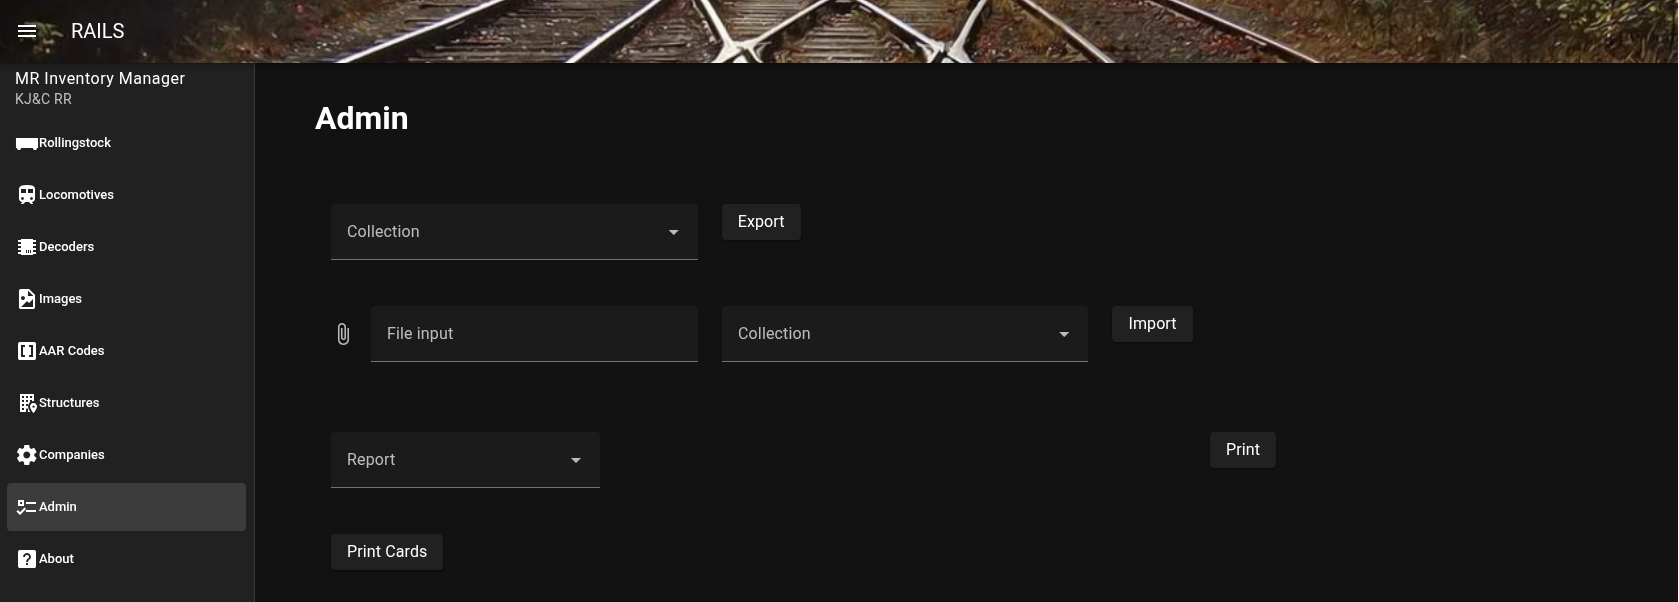
\includegraphics[width=0.85\textwidth]{./images/admin.png}
    \caption{Admin Page}
    \label{fig:admin}
\end{figure}

\subsection{Exporting Data Collections}

The Export control allows backup or data extraction of individual system collections. Selecting the "Collection" dropdown opens a list of available data sets, including AAR Codes, Companies, Images, Rolling Stock, Decoders, and Structures. Figure \ref{fig:admin-ex-collection} illustrates the collection selection menu for data export.

\begin{figure}[H]
    \centering
    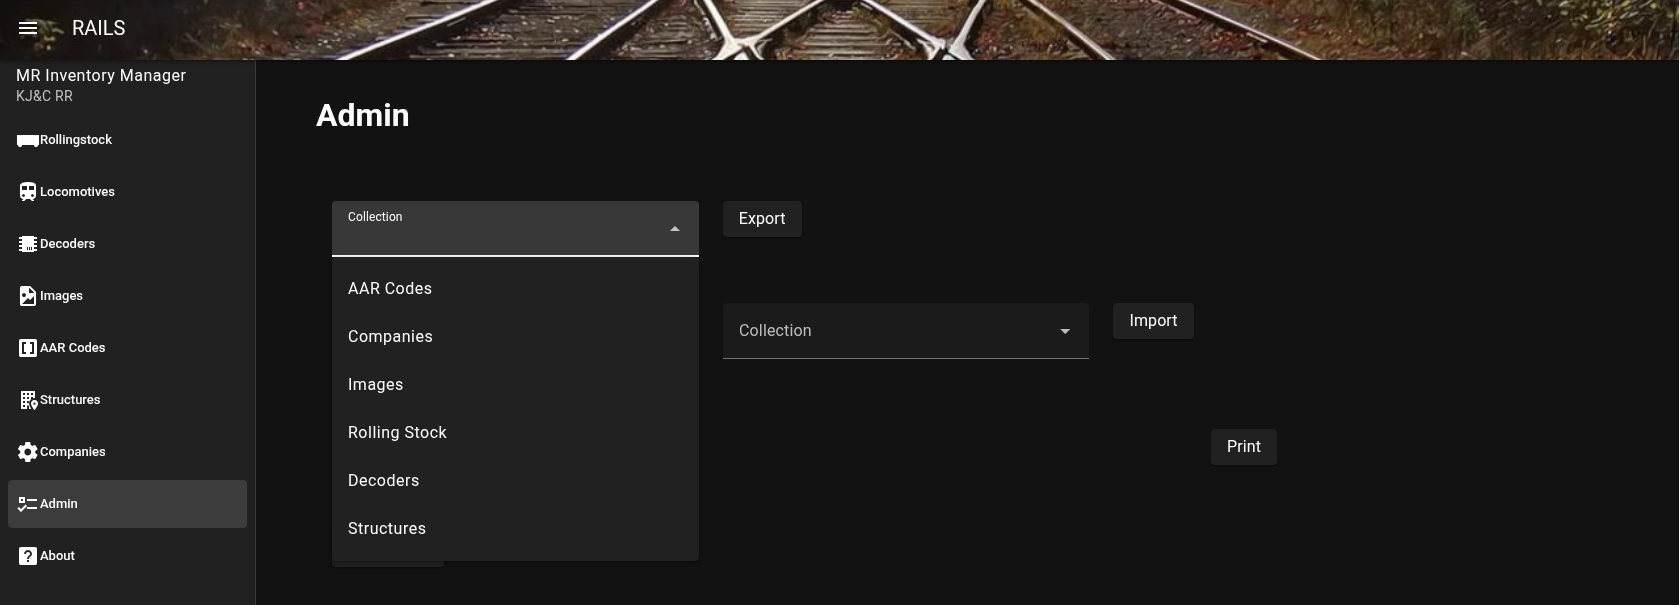
\includegraphics[width=0.85\textwidth]{./images/admin-ex-collection.png}
    \caption{Select Export Collection}
    \label{fig:admin-ex-collection}
\end{figure}

\subsection{Importing Data Collections}

To restore or bulk-load records, click the paperclip icon or file input field to launch the system file browser and select a local source file. Figure \ref{fig:admin-in-file} shows the native file chooser selection dialog.

\begin{figure}[H]
    \centering
    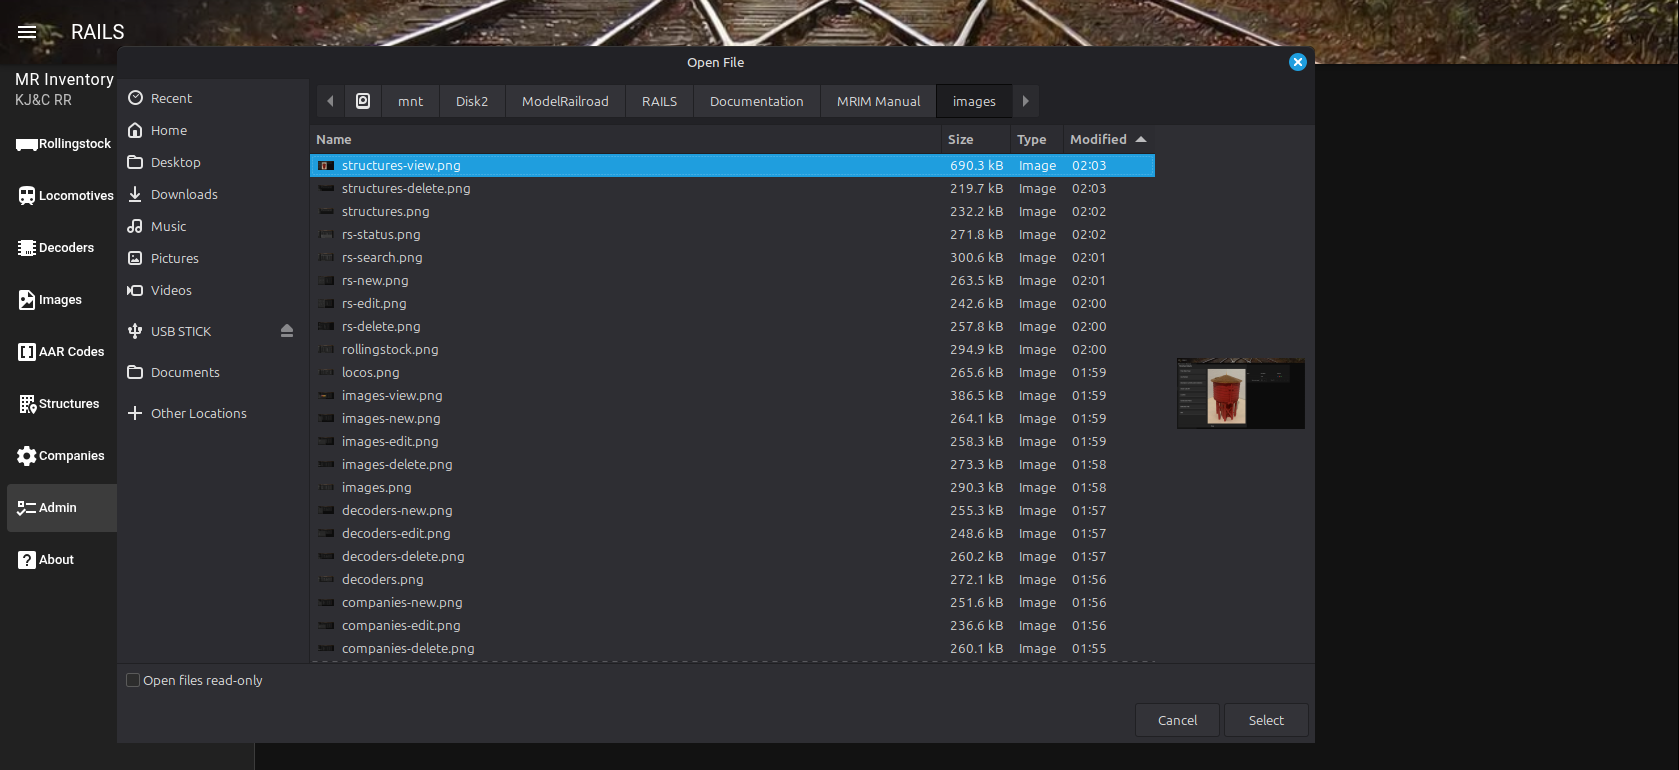
\includegraphics[width=0.85\textwidth]{./images/admin-in-file.png}
    \caption{Select Import Source File}
    \label{fig:admin-in-file}
\end{figure}

After specifying a source file, select the target database destination using the "Collection" dropdown menu. Options include AAR Codes, Companies, Images, Rolling Stock, Decoders, and Structures. Figure \ref{fig:admin-in-collection} illustrates selecting the target import collection before clicking "Import".

\begin{figure}[H]
    \centering
    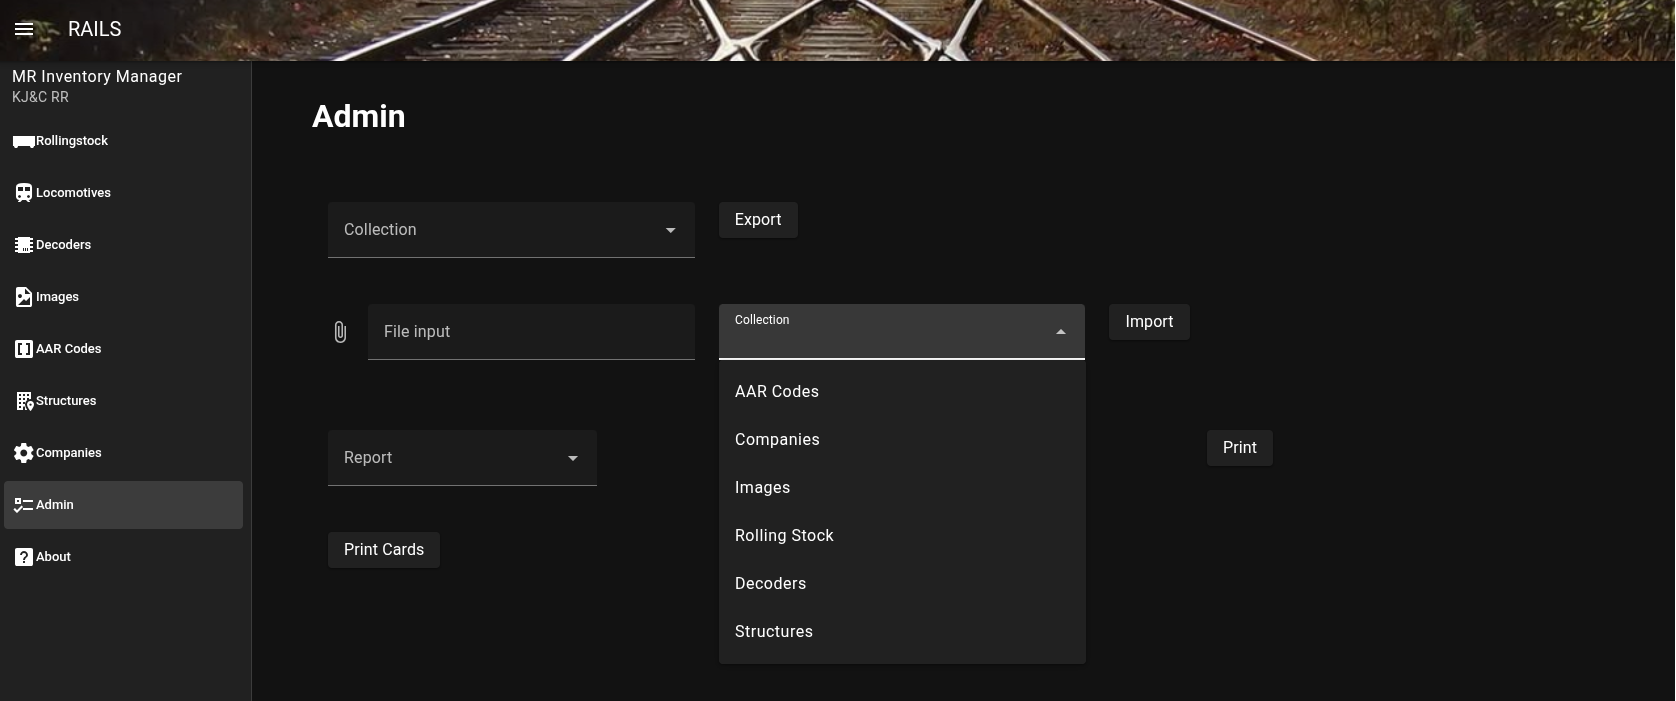
\includegraphics[width=0.85\textwidth]{./images/admin-in-collection.png}
    \caption{Select Target Import Collection}
    \label{fig:admin-in-collection}
\end{figure}

\subsection{Generating System Reports}

The Report section generates formatted system documentation and operational materials as a \gls{pdf} format. Selecting the "Report" dropdown displays available system inventories and assets for export, such as Rolling Stock, AAR Codes, Companies, Images, RFID, and Structures. Figure \ref{fig:admin-report} shows the report type selection menu.

\begin{figure}[H]
    \centering
    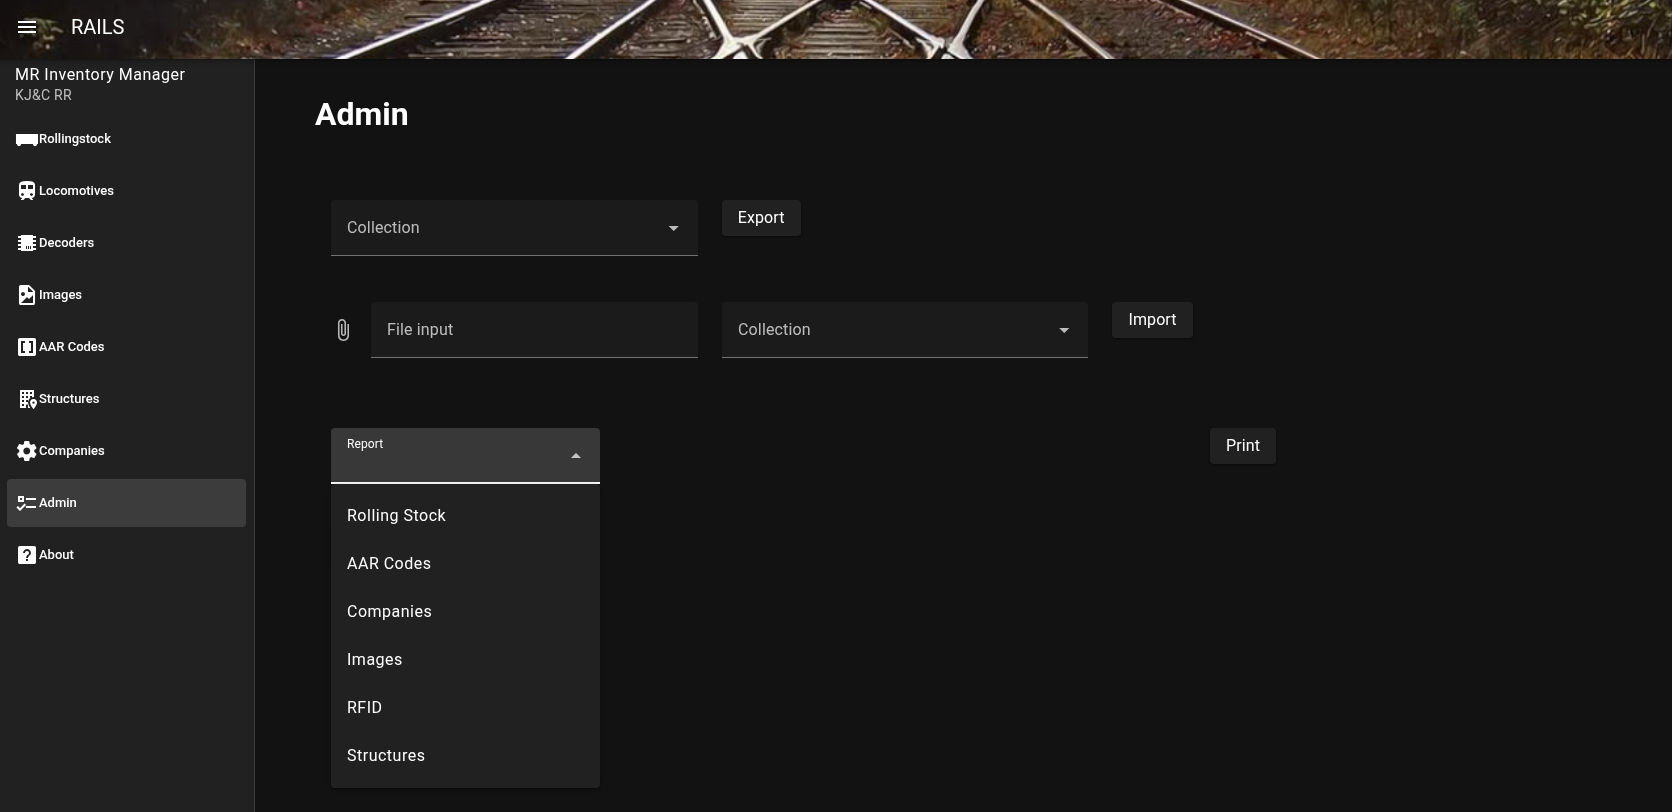
\includegraphics[width=0.85\textwidth]{./images/admin-report.png}
    \caption{Select Report Category}
    \label{fig:admin-report}
\end{figure}

When a specific report category like Rolling Stock is selected, additional sorting options appear. Clicking the "Sorted By" dropdown allows records to be ordered by parameters such as Road Names, AAR Codes, or Status. Figure \ref{fig:admin-rpt-rs-sort} illustrates the sorting criteria options.

\begin{figure}[H]
    \centering
    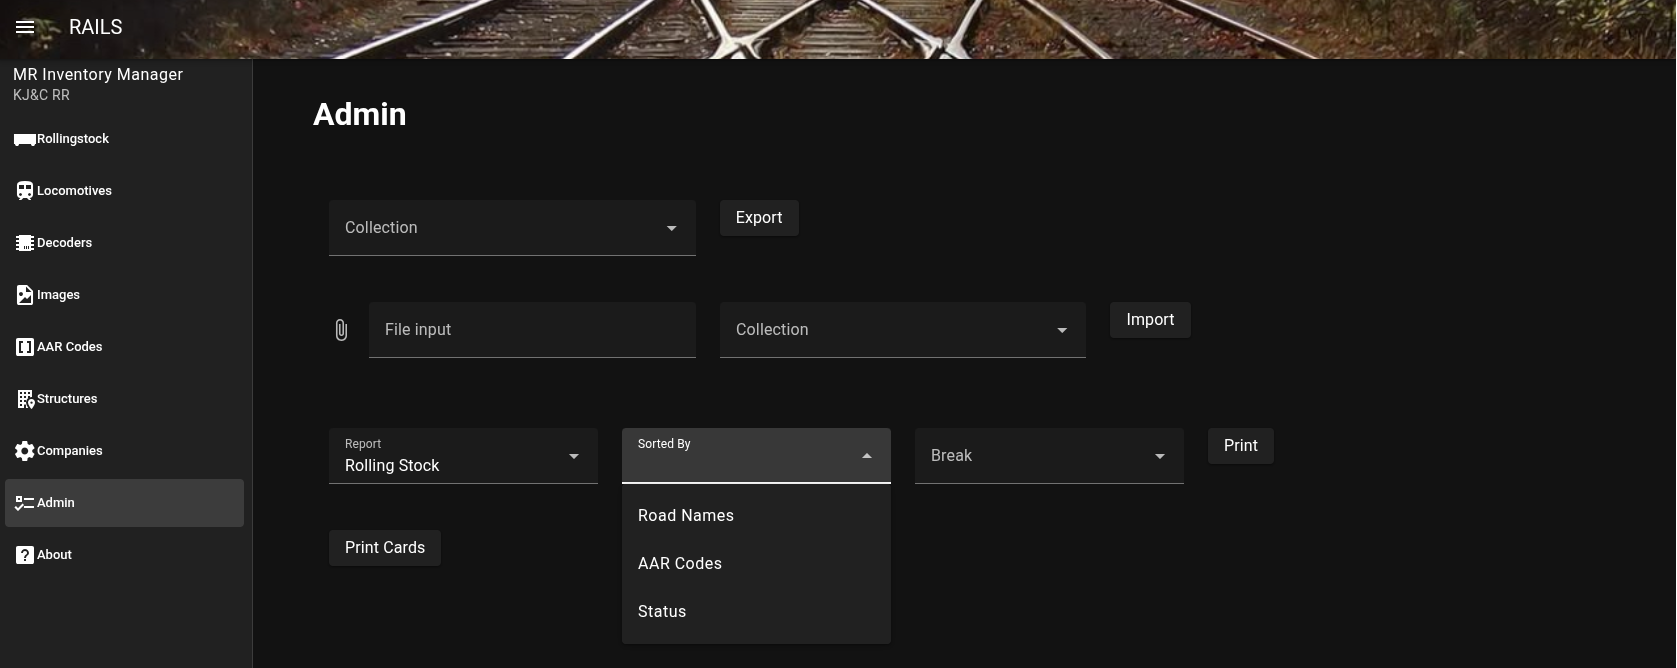
\includegraphics[width=0.85\textwidth]{./images/admin-rpt-rs-sort.png}
    \caption{Report Sort Options}
    \label{fig:admin-rpt-rs-sort}
\end{figure}

Reports can also be structured using page breaks or formatting style options. Selecting the "Break" dropdown provides options for Continuous formatting, Table views, or explicit Page breaks between sections. Figure \ref{fig:admin-rpt-rs-breaki} shows the report page break selection menu.

\begin{figure}[H]
    \centering
    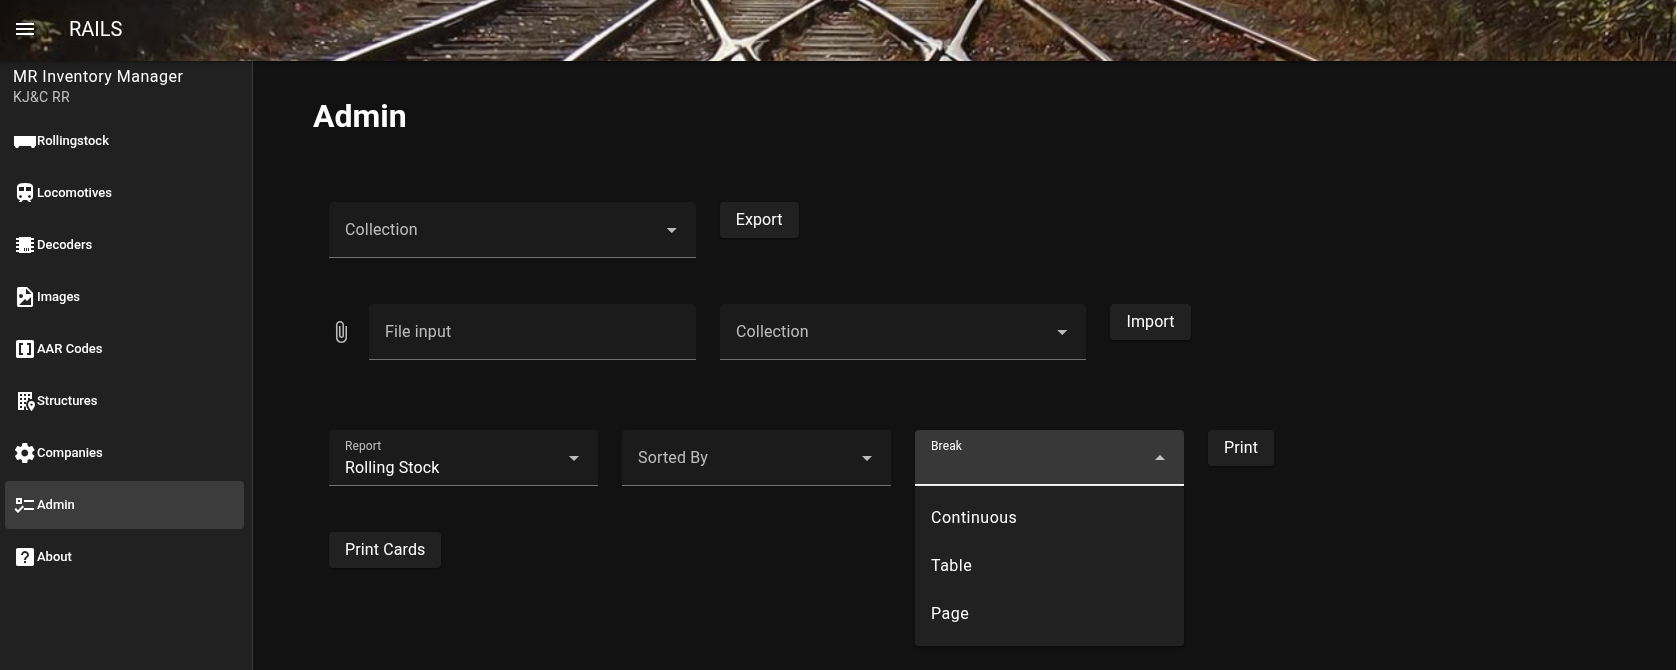
\includegraphics[width=0.85\textwidth]{./images/admin-rpt-rs-breaki.png}
    \caption{Report Page Break Formatting}
    \label{fig:admin-rpt-rs-breaki}
\end{figure}

Clicking on the "Print Cards" creates a set of pages that canbe cut into car cards used as a two-part system to track freight cars and simulate real-world cargo movements across a layout.
